%\documentclass{article}
%\usepackage{graphicx,subfigure}
%\begin{document}

\begin{figure}[!h]
  \centering
  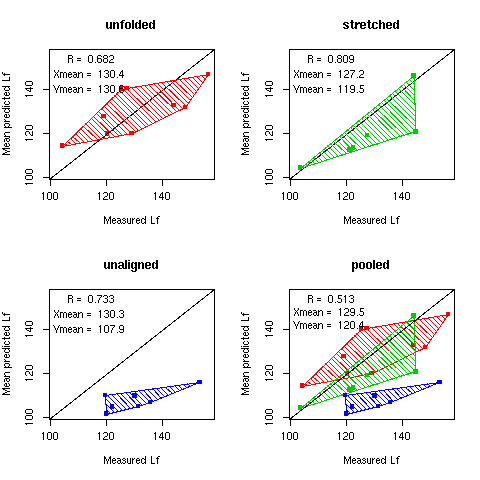
\includegraphics[width=1.1\textwidth]{figispredlf.png}
% original is nis.5.10.predlf.lf.png
  \caption{Plots of measured fibre length against predicted mean fibre length using Method 2 with predictions based on measurement of wavelength and amplitude by the {\em in-staple} technique, and crimps per staple calculated by equation ~\ref{eqn:T}. Fibre lengths for the unfolded crimp type wools were adjusted for the effect of twist at the points of inflection using $H = 0.5 * amplitude$ and $R = 0.10 mm$ in equation ~\ref{eqn:lf}.}
  \label{fig:ispredlf}
\end{figure}

%\end{document}

